\documentclass[10pt]{article}
\usepackage{tikz}
\usetikzlibrary{shapes.misc}
\usepackage[margin=0cm]{geometry}
\pagestyle{empty}
\tikzstyle{every node}=[cross out, draw, red]

\begin{document}

\vspace*{\fill}
\begin{center}
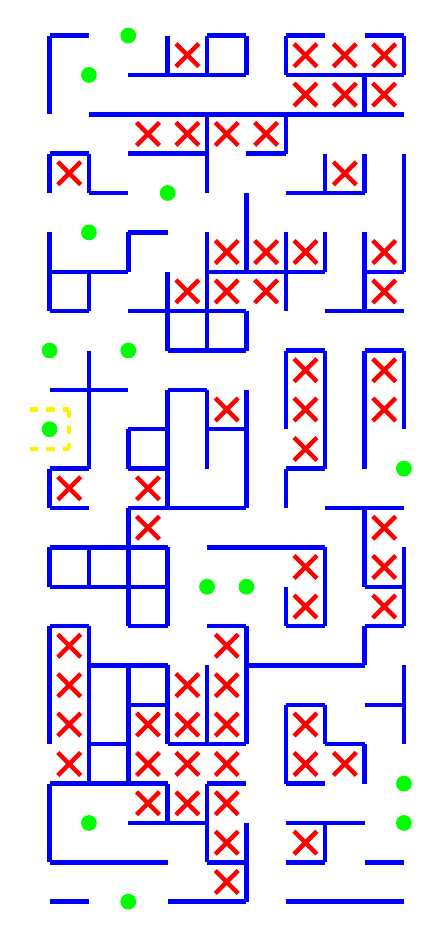
\begin{tikzpicture}[x=0.5cm, y=-0.5cm, ultra thick, blue]
% Walls
    \draw (0,0) -- (1,0);
    \draw (4,0) -- (5,0);
    \draw (6,0) -- (7,0);
    \draw (8,0) -- (9,0);
    \draw (2,1) -- (5,1);
    \draw (6,1) -- (9,1);
    \draw (1,2) -- (9,2);
    \draw (0,3) -- (1,3);
    \draw (2,3) -- (4,3);
    \draw (5,3) -- (6,3);
    \draw (1,4) -- (2,4);
    \draw (6,4) -- (8,4);
    \draw (2,5) -- (3,5);
    \draw (0,6) -- (2,6);
    \draw (4,6) -- (7,6);
    \draw (8,6) -- (9,6);
    \draw (0,7) -- (1,7);
    \draw (2,7) -- (5,7);
    \draw (7,7) -- (9,7);
    \draw (3,8) -- (5,8);
    \draw (6,8) -- (7,8);
    \draw (8,8) -- (9,8);
    \draw (0,9) -- (2,9);
    \draw (3,9) -- (4,9);
    \draw (2,10) -- (3,10);
    \draw (4,10) -- (5,10);
    \draw (0,11) -- (1,11);
    \draw (2,11) -- (3,11);
    \draw (6,11) -- (7,11);
    \draw (0,12) -- (1,12);
    \draw (2,12) -- (5,12);
    \draw (7,12) -- (9,12);
    \draw (0,13) -- (3,13);
    \draw (4,13) -- (7,13);
    \draw (0,14) -- (3,14);
    \draw (8,14) -- (9,14);
    \draw (0,15) -- (1,15);
    \draw (2,15) -- (3,15);
    \draw (4,15) -- (5,15);
    \draw (6,15) -- (7,15);
    \draw (8,15) -- (9,15);
    \draw (1,16) -- (3,16);
    \draw (5,16) -- (8,16);
    \draw (2,17) -- (3,17);
    \draw (6,17) -- (7,17);
    \draw (8,17) -- (9,17);
    \draw (1,18) -- (2,18);
    \draw (3,18) -- (5,18);
    \draw (7,18) -- (8,18);
    \draw (0,19) -- (3,19);
    \draw (4,19) -- (5,19);
    \draw (6,19) -- (7,19);
    \draw (2,20) -- (4,20);
    \draw (6,20) -- (8,20);
    \draw (0,21) -- (3,21);
    \draw (4,21) -- (5,21);
    \draw (6,21) -- (7,21);
    \draw (8,21) -- (9,21);
    \draw (0,22) -- (1,22);
    \draw (3,22) -- (5,22);
    \draw (6,22) -- (9,22);
    \draw (0,0) -- (0,2);
    \draw (0,3) -- (0,4);
    \draw (0,5) -- (0,7);
    \draw (0,11) -- (0,12);
    \draw (0,13) -- (0,14);
    \draw (0,15) -- (0,18);
    \draw (0,19) -- (0,21);
    \draw (1,3) -- (1,4);
    \draw (1,6) -- (1,7);
    \draw (1,8) -- (1,11);
    \draw (1,13) -- (1,14);
    \draw (1,15) -- (1,19);
    \draw (2,5) -- (2,6);
    \draw (2,10) -- (2,11);
    \draw (2,12) -- (2,15);
    \draw (2,16) -- (2,19);
    \draw (3,0) -- (3,1);
    \draw (3,6) -- (3,8);
    \draw (3,9) -- (3,12);
    \draw (3,13) -- (3,15);
    \draw (3,16) -- (3,18);
    \draw (3,19) -- (3,20);
    \draw (4,0) -- (4,1);
    \draw (4,2) -- (4,4);
    \draw (4,5) -- (4,8);
    \draw (4,9) -- (4,11);
    \draw (4,16) -- (4,18);
    \draw (4,19) -- (4,21);
    \draw (5,0) -- (5,1);
    \draw (5,4) -- (5,6);
    \draw (5,7) -- (5,8);
    \draw (5,9) -- (5,12);
    \draw (5,15) -- (5,18);
    \draw (5,20) -- (5,22);
    \draw (6,0) -- (6,1);
    \draw (6,2) -- (6,3);
    \draw (6,5) -- (6,7);
    \draw (6,8) -- (6,10);
    \draw (6,11) -- (6,12);
    \draw (6,14) -- (6,15);
    \draw (6,17) -- (6,19);
    \draw (7,3) -- (7,4);
    \draw (7,5) -- (7,6);
    \draw (7,8) -- (7,11);
    \draw (7,13) -- (7,15);
    \draw (7,17) -- (7,18);
    \draw (7,20) -- (7,21);
    \draw (8,1) -- (8,2);
    \draw (8,3) -- (8,4);
    \draw (8,5) -- (8,7);
    \draw (8,8) -- (8,11);
    \draw (8,12) -- (8,14);
    \draw (8,15) -- (8,16);
    \draw (8,18) -- (8,19);
    \draw (9,0) -- (9,1);
    \draw (9,3) -- (9,6);
    \draw (9,8) -- (9,10);
    \draw (9,13) -- (9,15);
    \draw (9,16) -- (9,18);
% Pillars
    \fill[green] (2,0) circle(0.2);
    \fill[green] (1,1) circle(0.2);
    \fill[green] (3,4) circle(0.2);
    \fill[green] (1,5) circle(0.2);
    \fill[green] (0,8) circle(0.2);
    \fill[green] (2,8) circle(0.2);
    \fill[green] (0,10) circle(0.2);
    \fill[green] (9,11) circle(0.2);
    \fill[green] (4,14) circle(0.2);
    \fill[green] (5,14) circle(0.2);
    \fill[green] (9,19) circle(0.2);
    \fill[green] (1,20) circle(0.2);
    \fill[green] (9,20) circle(0.2);
    \fill[green] (2,22) circle(0.2);
% Inner points in accessible cul-de-sacs
    \node at (3.5,0.5) {};
    \node at (6.5,0.5) {};
    \node at (7.5,0.5) {};
    \node at (8.5,0.5) {};
    \node at (6.5,1.5) {};
    \node at (7.5,1.5) {};
    \node at (8.5,1.5) {};
    \node at (2.5,2.5) {};
    \node at (3.5,2.5) {};
    \node at (4.5,2.5) {};
    \node at (5.5,2.5) {};
    \node at (0.5,3.5) {};
    \node at (7.5,3.5) {};
    \node at (4.5,5.5) {};
    \node at (5.5,5.5) {};
    \node at (6.5,5.5) {};
    \node at (8.5,5.5) {};
    \node at (3.5,6.5) {};
    \node at (4.5,6.5) {};
    \node at (5.5,6.5) {};
    \node at (8.5,6.5) {};
    \node at (6.5,8.5) {};
    \node at (8.5,8.5) {};
    \node at (4.5,9.5) {};
    \node at (6.5,9.5) {};
    \node at (8.5,9.5) {};
    \node at (6.5,10.5) {};
    \node at (0.5,11.5) {};
    \node at (2.5,11.5) {};
    \node at (2.5,12.5) {};
    \node at (8.5,12.5) {};
    \node at (6.5,13.5) {};
    \node at (8.5,13.5) {};
    \node at (6.5,14.5) {};
    \node at (8.5,14.5) {};
    \node at (0.5,15.5) {};
    \node at (4.5,15.5) {};
    \node at (0.5,16.5) {};
    \node at (3.5,16.5) {};
    \node at (4.5,16.5) {};
    \node at (0.5,17.5) {};
    \node at (2.5,17.5) {};
    \node at (3.5,17.5) {};
    \node at (4.5,17.5) {};
    \node at (6.5,17.5) {};
    \node at (0.5,18.5) {};
    \node at (2.5,18.5) {};
    \node at (3.5,18.5) {};
    \node at (4.5,18.5) {};
    \node at (6.5,18.5) {};
    \node at (7.5,18.5) {};
    \node at (2.5,19.5) {};
    \node at (3.5,19.5) {};
    \node at (4.5,19.5) {};
    \node at (4.5,20.5) {};
    \node at (6.5,20.5) {};
    \node at (4.5,21.5) {};
% Entry-exit paths without intersections
    \draw[dashed, yellow] (-0.5,9.5) -- (0.5,9.5);
    \draw[dashed, yellow] (-0.5,10.5) -- (0.5,10.5);
    \draw[dashed, yellow] (0.5,9.5) -- (0.5,10.5);
\end{tikzpicture}
\end{center}
\vspace*{\fill}

\end{document}
